%%% LaTeX Template: Article/Thesis/etc. with colored headings and special fonts
%%%
%%% Source: http://www.howtotex.com/

\documentclass[12pt]{article}


\usepackage{apuntes-estilo}
\usepackage{fancyhdr,lastpage}
\usepackage{color,colortbl}
\usepackage{verbatim}

\def\maketitle{

% Titulo 
 \makeatletter
 {\color{bl} \centering \huge \sc \textbf{
 Manteniendo la hora \\ 
\large \vspace*{-8pt} \color{black} Guía básica de mantenimiento de la hora
 \vspace*{8pt} }\par}
 \makeatother


% Autor
 \makeatletter
 {\centering \small 
 	Departamento de Ingeniería de Computadoras \\
 	Facultad de Informática - Universidad Nacional del Comahue \\
 	\vspace{20pt} }
 \makeatother

}

% Custom headers and footers
\fancyhf{} % clear all header and footer fields
\fancypagestyle{plain}{\fancyhf{}}
  	\pagestyle{fancy}
 	\lhead{\footnotesize Manteniendo la hora - Departamento de Ingeniería de Computadoras}
 	\rhead{\footnotesize \thepage\ }	% ''Page 1 of 2''

\def\ti#1#2{\texttt{#1} & #2 \\ }



\begin{document}

\thispagestyle{empty}
\maketitle
\setlength{\parindent}{0pt}

\section*{ Manteniendo La Hora}

En este capítulo se explica como un sistema Linux mantiene la fecha y hora,
y lo que debe conocer para evitar problemas. Si bien el mantenimiento de
la hora no es una actividad frecuente, es responsabilidad del administrador 
del sistema realizar los cambios que sean necesarios. 


\subsection*{Zonas horarias}

Las mediciones horarias están basadas en su mayoría a fenómenos naturales regulares,
como por ejemplo, los periodos alternados de luz y oscuridad
causados por la rotación del planeta. El tiempo total tomado por dos períodos
sucesivos es constante, pero la duración del período de luz varía
con respecto al de oscuridad. Una constante simple es la luz del mediodía.

El mediodía es el momento del día en el cual el Sol se encuentra en la posición más alta. 
Debido a la rotación de la Tierra, el momento del mediodía sucede en diferentes 
momentos en diferentes lugares. Esto nos conduce al concepto de \textit{hora local}.
Si permanecemos siempre en el mismo lugar, las diferencias entre los
horarios locales de diferentes sitios pareciera no tienen mucha importancia.

Sin embargo, en cuanto necesite comunicarse con lugares distantes, con horarios locales 
diferentes, notará la necesidad de una hora en común. Hoy en día, la mayoría de los lugares en el mundo deben
comunicarse con otros, por lo que se definió un estándar mundial de medición
horaria. Este estándar se llama \textit{hora universal} ó UTC (del inglés Universal 
Time Coordinated), y es uno de los varios sucesores estrechamente 
relacionados con el tiempo medio de Greenwich (GMT). De hecho, aunque técnicamente 
difieren GMT y UTC suelen utilizarse como sinónimos en mucha bibliografía.   
De este modo, cuando personas con diferentes horas locales
necesitan comunicarse, pueden expresar el tiempo en hora universal,
para que no exista confusión acerca de cuándo deben suceder las cosas.

Cada hora local es llamada zona horaria (time zone), y existen 24 zonas horarias
en el planeta. Si bien geográficamente es posible pensar que todos los lugares
en donde el mediodía suceda en el mismo momento tienen la misma zona horaria,
políticamente esto no siempre así. Por diversas razones, varios países
adoptan el ``horario de verano'' (\textit{daylight savings time} o DST) para atender las demandas
económicas. Los países que adoptan el ``horario de verano'' cambian la hora
de sus relojes en verano (en general. se retrasan los relojes una hora) para
tener más luz natural mientras trabajan (durante la tarde), y vuelven a adelantar
la hora de sus relojes en otoño o invierno. Otros países no adoptan estos procedimientos.
Más aún, los países que utilizan horarios de verano no tienen un acuerdo común de cuándo deben
modificarse los relojes, y cambian, además, las reglas año tras año. Por lo que las
conversiones de zonas horarias son definitivamente no-triviales.

\begin{center}
 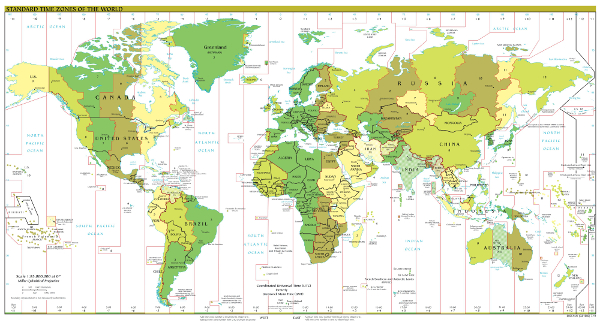
\includegraphics{World_Time_Zones_Map.jpg}
\end{center}

Las zonas horarias son denominadas de mejor manera a través de su ubicación o por
la diferencia entre la hora universal y la hora local. En la Argentina y
en algunos otros países, las zonas horarias locales tienen un nombre y una abreviatura
de tres letras (ART en nuestro caso). Las abreviaturas \textbf{no son únicas}, por lo que no deberían
ser utilizadas sin que aparezca también el nombre del país. Es mejor referirse a la
la hora local en Helsinki, que referirse a la hora del Este de Europa, debido a que
no todos los países del Este de Europa adoptan las mismas reglas. De hecho dentro 
de nuestro país, Argentina,  ha sucedido que diferentes provincias utilicen diferentes
zonas horarias. \footnote{Ver http://es.wikipedia.org/wiki/Hora\_oficial\_argentina}


GNU/Linux tiene un paquete de zonas horarias que reconoce todas las zonas horarias existentes,
y puede ser fácilmente actualizado cuando las reglas cambian. Todo lo que un administrador de 
sistemas necesita hacer es seleccionar la zona horaria apropiada. A su vez, cada usuario 
puede establecer su propia zona horaria (recordemos que GNU/Linux es un sistema multiusuario); 
por lo que facilita el trabajo de mucha gente, debido a que muchas personas trabajan en diferentes 
países a través de Internet y quizá sobre el mismo equipo.
Cuando las reglas del ``horario de verano'' cambian para el horario local de los equipos que 
administra, asegúrese de actualizar al menos la zona horaria del sistema y de ser necesario 
la definición de zonas horarias disponibles. 


\subsection*{Los relojes de software y hardware}


En general las computadoras tiene un reloj de hardware alimentado por una batería, conocido también como 
``reloj de tiempo real'' o RTC (del inglés \textit{Real Time Clock}). 
Esa batería asegura que el reloj continúe trabajando aún cuando la computadora se encuentre sin
suministro eléctrico. El reloj de hardware puede ser modificado (o definido)
desde el firmware inicial que controla la placa base, como por ejemplo el BIOS en las 
computadoras personales, o desde cualquier sistema operativo.

Por otra parte, una vez iniciado el sistema, el kernel Linux mantiene la fecha y hora 
de manera independiente al reloj de hardware. Este reloj es conocido como ``reloj de sistema'', 
``reloj de software'' o ``reloj del kernel''. 
Durante el inicio de un sistema Linux, el kernel configura su propio reloj de software accediendo
a la fecha y hora mantenida por el reloj de hardware.
Luego, ambos relojes trabajan independientemente.
Linux mantiene su propio reloj debido a que leer el reloj de hardware constantemente es 
lento, complicado e inexacto.

El reloj del kernel siempre muestra la hora universal, por lo que
no necesita conocer como utilizar husos horarios. La simplicidad de este
modo de trabajar proporciona alta confiabilidad y facilita actualizar 
la información de la zona horaria. Cada proceso realiza las conversiones de zona horaria 
de manera independiente (utilizando herramientas estándar que son parte del paquete de zona horaria).


El reloj de hardware puede estar en formato de hora local u hora universal.
Usualmente es mejor que el reloj de hardware mantenga la hora universal,
porque de esta manera no será necesario modificar la hora del reloj cuando el ``horario de verano''
(daylight savings time o DST) empiece o finalice (UTC no tiene DST). Desafortunadamente, algunos sistemas operativos 
(por ejemplo MS-DOS, Windows y OS/2) asumen que el reloj de hardware muestra la hora local.
Por otra parte, Linux puede manejar cualquiera de los dos formatos, pero si el reloj de hardware muestra la hora local,
entonces debe modificarlo cada vez que el ``horario de verano'' empiece o finalice. Este 
punto es particularmente conflictivo en equipos donde coexisten más de un 
sistema operativo (clásico dual boot Windows-GNU/Linux). 


\subsection*{Configurar y visualizar la hora}

En Linux, la zona horaria del sistema es determinada por \texttt{/etc/localtime} (algunas veces
es un enlace simbólico). Si es un enlace, entonces apunta a un archivo de datos de zona horaria
que describe la zona horaria local. Los archivos de datos de zonas horarias están ubicados en
\texttt{/usr/lib/zoneinfo} o \texttt{/usr/share/zoneinfo}. (Esto puede variar según la 
distribución particular de GNU/Linux utilizada). 

Por ejemplo, en un sistema SuSE ubicado en Santiago de Chile \texttt{/etc/localtime} apuntaría
a \texttt{/usr/share/zoneinfo/Chile/Continental (UTC-4)}.

Si no encuentra el directorio \texttt{zoneinfo} en \texttt{/usr/lib} o en \texttt{/usr/share}, 
intente encontrarlo ejecutando \texttt{\textbf{find /usr -type d -name zoneinfo}}, o consulte 
la documentación de su distribución GNU/Linux particular.

\textbf{Múltiples usuarios en diferentes zonas horarias:}

¿Qué sucede cuando existen usuarios utilizando el mismo sistema pero se encuentran ubicados en
zonas horarias diferentes?
Un usuario puede cambiar su zona horaria privada definiendo la variable de ambiente TZ.
Si TZ no se encuentra definida, entonces la zona horaria del sistema es la utilizada.
La sintaxis de la variable TZ se encuentra descripta en la página de manual de \texttt{\textbf{tzset}}.


\colorbox{grey}{\parbox[t]{0.95\linewidth}{ \vspace*{0.5cm} { 
Por ejemplo si la hora local del sistema esta definida para Argentina, tal que 
el comando \texttt{date} nos devuelve: \\
{\tt\# date \\
mié jul 31 17:14:40 ART 2013} \\
Y ahora definimos la variable de ambiente TZ con el valor (Eastern Standard Time, utilizada en 
algunas regiones de Estados Unidos), veremos que la salida de \texttt{date} responde 
a la nueva hora local utilizada por el usuario: \\
{\tt
\# export TZ=EST \\
\# date \\
mié jul 31 15:14:53 EST 2013 \\
} 
Esto es, dos horas de diferencia con la hora local Argentina. 
 } \vspace*{0.5cm} } } 

Algunas distribuciones proveen el comando \texttt{tzselec} para ayudar al usuario a 
identificar el valor que debiera utilizar para la variable TZ.

\colorbox{grey}{\parbox[t]{0.95\linewidth}{ \vspace*{0.5cm} { 
{\tt 
\# tzselect \\
Please identify a location so that time zone rules can be set correctly.\\
Please select a continent or ocean.\\
 1) Africa\\
 2) Americas\\
 3) Antarctica\\
 4) Arctic Ocean\\
 5) Asia\\
 6) Atlantic Ocean\\
 7) Australia\\
 8) Europe\\
 9) Indian Ocean\\
10) Pacific Ocean\\
11) none - I want to specify the time zone using the Posix TZ format.\\
\#? 1\\
}
 } \vspace*{0.5cm} } } 


\colorbox{grey}{\parbox[t]{0.95\linewidth}{ \vspace*{0.5cm} { 
{\tt 
Please select a country.\\
 1) Algeria		  18) Gabon		    35) Rwanda\\
 2) Angola		  19) Gambia		    36) Sao Tome \& Principe\\
 3) Benin		  20) Ghana		    37) Senegal\\
 4) Botswana		  21) Guinea		    38) Sierra Leone\\
 5) Burkina Faso	  22) Guinea-Bissau	    39) Somalia\\
 6) Burundi		  23) Kenya		    40) South Africa\\
 7) Cameroon		  24) Lesotho		    41) South Sudan\\
 8) Central African Rep.  25) Liberia		    42) Spain\\
 9) Chad		  26) Libya		    43) Sudan\\
10) Congo (Dem. Rep.)	  27) Malawi		    44) Swaziland\\
11) Congo (Rep.)	  28) Mali		    45) Tanzania\\
12) Cote d'Ivoire	  29) Mauritania	    46) Togo\\
13) Djibouti		  30) Morocco		    47) Tunisia\\
14) Egypt		  31) Mozambique	    48) Uganda\\
15) Equatorial Guinea	  32) Namibia		    49) Western Sahara\\
16) Eritrea		  33) Niger		    50) Zambia\\
17) Ethiopia		  34) Nigeria		    51) Zimbabwe\\
\#? 2\\
\\
The following information has been given:\\
\\
	Angola\\
\\
Therefore TZ='Africa/Luanda' will be used.\\
Local time is now:	Mon Aug  5 14:29:57 WAT 2013.\\
Universal Time is now:	Mon Aug  5 13:29:57 UTC 2013.\\
Is the above information OK?\\
1) Yes\\
2) No\\
\#? 1\\
\\
You can make this change permanent for yourself by appending the line\\
	TZ='Africa/Luanda'; export TZ\\
to the file '.profile' in your home directory; then log out and log in again.\\
\\
Here is that TZ value again, this time on standard output so that you\\
can use the /usr/bin/tzselect command in shell scripts:\\
Africa/Luanda\\
\# TZ='Africa/Luanda'; export TZ\\
\# date\\
lun ago  5 14:30:26 WAT 2013\\
\# \\
}
 } \vspace*{0.5cm} } } 
\\ 
\\ 
\\ 
\textbf{El comando \texttt{\textbf{date}}}

El comando \texttt{\textbf{date}} muestra la hora y fecha actuales. Por ejemplo:

\colorbox{grey}{\parbox[t]{0.95\linewidth}{ \vspace*{0.5cm} {\tt 
\# date \\
mié jul 31 17:14:40 ART 2013
 } \vspace*{0.5cm} } } 

Es decir, miércoles 31 de julio del 2013, cinco y cuarto de la tarde en hora local Argentina  \textit{``ART''}.
El comando \texttt{\textbf{date}} también puede también mostrar la hora universal (UTC): 


\colorbox{grey}{\parbox[t]{0.95\linewidth}{ \vspace*{0.5cm} {\tt 
\# date -u\\
mié jul 31 20:18:02 UTC 2013
 } \vspace*{0.5cm} } } 


\texttt{\textbf{date}} también se utiliza para establecer la hora del \textit{reloj del kernel}. Para más información
lea la página de manual de \texttt{\textbf{date}}. Tenga en cuenta que \textbf{solo el usuario root puede 
modificar la fecha y/u hora del sistema}. Recuerde que si bien cada usuario puede definir su propia zona horaria, el reloj 
es el mismo para todos.

\colorbox{grey}{\parbox[t]{0.95\linewidth}{ \vspace*{0.5cm}
En el siguiente ejemplo se modifica la hora y fecha del reloj del kernel 
utilizando el comando date: \\
{\tt 
\# date 08051657 \\
lun ago  5 16:57:00 ART 2013
 } \vspace*{0.5cm} } } 

\textbf{El comando \texttt{hwclock}}

Como vimos, \texttt{\textbf{date}} muestra o modifica el reloj de software. 
Por otra parte, todas las distribuciones GNU/Linux proveen el comando \texttt{clock} o su reemplazo más
reciente \texttt{hwclock} (utilizaremos este último en el resto del texto). Dichos comandos permiten 
sincronizar los relojes de hardware y software. Cuando el sistema inicia, el comando \texttt{hwclock}
 es utilizado para leer el reloj de hardware y actualizar el reloj de software. La forma en que el 
sistema lleva a cabo esta tarea varía entre distribuciones. 

\colorbox{grey}{\parbox[t]{0.95\linewidth}{ \vspace*{0.5cm}
Por ejemplo en el caso particular de Debian esto se hace a través de un script de inicio ubicado 
en /etc/init.d y un archivo de configuración /etc/default/hwclock que controla el comportamiento 
de dicho script: \\
{\tt
find /etc -iname "*hwclock*"\\
/etc/rcS.d/S05hwclock.sh\\
/etc/init.d/hwclock.sh\\
/etc/rc0.d/K08hwclock.sh\\
/etc/rc6.d/K08hwclock.sh\\
/etc/default/hwclock\\
}
Otros lugares comunes para efectuar la sincronización en el arranque son /etc/rc.local, 
/etc/rc.d/rc.sysinit, /etc/rc.d/boot, entre otros. 
} \vspace*{0.5cm} }  

Si necesita modificar ambos relojes (software y hardware), primero debe modificar el 
reloj de software con \texttt{\textbf{date}}, y luego sincronizar la hora del reloj 
por hardware con el comando \texttt{\textbf{hwclock -w o hwclock --systohc}}.

La opción \texttt{ ``-u o --utc''} en el comando \texttt{\textbf{hwclock}} le indica 
a \texttt{hwclock} que la fecha y hora (mostrada o definida)
se encuentra en formato de hora universal (UTC). \textit{Debe} utilizar la opción -u correctamente, en
caso contrario el efecto sobre la hora del sistema puede no ser el esperado. 


Los relojes deben modificarse con cuidado y precisión.
Algunas partes de un sistema UNIX requieren que los relojes trabajen correctamente.
Por ejemplo, el demonio \texttt{\textbf{cron}} ejecuta comandos periódicamente basándose en la
hora y día para ello. Si cambia el reloj, el sistema puede tomar decisiones no previstas por 
el administrador en cuanto a la necesidad o no de ejecutar determinado comando.
En general grandes saltos en el tiempo (hacia el futuro o el pasado) pueden causar conflictos mayores
que pequeñas diferencias.



\section*{NTP - Protocolo de red para sincronización de reloj}

Alternativamente a revisar periódicamente el reloj del kernel y ajustarlo 
manualmente, una computadora conectada en red puede 
comprobar su propio reloj de forma automática, comparándolo con la hora
de otro ordenador que se sabe almacena la hora de forma precisa. El 
protocolo de tiempo en red (o NTP) hace esto exactamente. Es un método para 
verificar y corregir la hora de su computadora al sincronizarse con otro 
sistema. Con NTP su sistema puede mantenerse a milisegundos de la Hora 
Universal Coordinada (UTC). 
	
Para la mayoría de usuarios ocasionales de Linux, esto puede parecer
simplemente un lujo.  Para grandes organizaciones 
este ``lujo'' puede convertirse en fundamental. Por ejemplo, ser capaz de 
buscar sucesos en los archivos de bitácora (log) basándose en la hora puede hacer la vida 
bastante más sencilla y puede eliminar mucho ``trabajo de adivinación'' 
durante la depuración.

En diversos software de clustering, esto es software que implementa el trabajo 
en equipo entre dos o más computadoras, la sincronización de relojes es 
clave para el correcto funcionamiento del software. Muchas de las actividades 
en las que las computadoras pertenecientes a un cluster (grupo de trabajo)
se ponen de acuerdo están basadas en el tiempo.

Dentro de un centro de cómputos, existen múltiples ejemplos en los que la 
exactitud del reloj es clave para el correcto funcionamiento. Por otra parte
debe tenerse en cuenta que, en muchos casos, lo importante es la sincronización de 
relojes entre máquinas en una misma red y no la exactitud con respecto a UTC, NTP 
esta pensado para tal fin.   


%Otro ejemplo de cuan importante puede ser NTP es con SAN. Algunos SAN
%necesitan NTP para configurarse y funcionar adecuadamente para permitir
%la correcta sincronización durante el uso del sistema de ficheros, y un
%control adecuado de las marcas de tiempo. Algunos SAN (y algunas
%aplicaciones) pueden confundirse cuando tratan con archivos que tienen marcas
%de tiempo que están en el futuro.


\subsection*{Configuración básica de NTP}

La mayoría de las distribuciones GNU/Linux proveen un paquete de software que implementa 
NTP. Puede utilizarlo para instalar NTP, o bien puede bajarse el código fuente de \\
http://www.ntp.org/downloads.html y compilarlo usted mismo. En
cualquier caso, la configuración básica es la misma.

El programa NTP, \texttt{ntpd} se configura utilizando el archivo \texttt{/etc/ntp.conf} o
\texttt{/etc/xntp.conf} \footnote{Xntp hace referencia a la vieja implementación 
NTPv3 que fue reemplazada por ntpd NTPv4} dependiendo de qué distribución Linux tenga. 
En dicho archivo se establece uno o mas \textit{servidores NTP} a los cuales 
consultar el reloj. 

Ejemplo de archivo ntp.conf básico: 

\colorbox{grey}{\parbox[t]{0.95\linewidth}{ \vspace*{0.5cm} {\tt
\# --- GENERAL CONFIGURATION --- \\
server  0.debian.pool.ntp.org \#nombre de dominio \\
server  142.54.181.202 \#IP v4 \\
server  127.127.1.0 \#local \\

\# Drift file.\\
driftfile /etc/ntp/drift
 } \vspace*{0.5cm} } } 

	
El archivo ntp.conf básico listará dos servidores, uno
con el que le gustaría sincronizarse, y una dirección pseudo-IP para él 
mismo (en este caso 127.127.1.0). La pseudo-IP se utiliza en el caso de
errores en la red o si cae el servidor NTP remoto. NTP sincronizará
consigo mismo hasta que pueda empezar a sincronizar de nuevo con el 
servidor remoto. Se recomienda que se pongan al menos dos servidores remotos
con los que pueda sincronizarse. Uno actuará como servidor primario y el 
otro en caso de fallo.

También debe ponerse una ubicación para el archivo de fluctuación (drift). De 
vez en cuando NTP \textit{aprenderá} el error que se comete en el reloj de
sistema (local) y automáticamente se ajustará.

NTP corrige el sistema lentamente. ¡Sea paciente! Una simple prueba es
cambiar el reloj de sistema en diez minutos antes de irse a la cama y
comprobarlo cuando se levante. La hora deberá ser la correcta.

\subsection*{NTP en el arranque: ntpd}
El software de NTP se inicia con el arranque del sistema. Usualmente encontraremos
un script the inicio en /etc/init.d o similar, dependiendo del sistema de servicios 
de su distribución particular, que ejecuta el binario \texttt{ntpd}.

\colorbox{grey}{\parbox[t]{0.95\linewidth}{ \vspace*{0.5cm} 
Por ejemplo en el caso de una distribución Debian encontramos los siguientes 
archivos en /etc: \\ 
{\tt
\# find /etc/ -iname "*ntp*"\\
/etc/rc2.d/S07ntp\\
/etc/rc5.d/S07ntp\\
/etc/rc4.d/S07ntp\\
/etc/rc3.d/S07ntp\\
/etc/init.d/ntp\\
/etc/ntp.conf\\
/etc/default/ntp\\
 } 
Observamos que existen scripts de inicio de ntp, luego si comprobamos los procesos en 
ejecución encontraremos a \texttt{ntpd} ejecutándose:\\ 
{\tt
\# ps -ef |grep ntpd\\
ntp       3719     1  0 jul28 ?        00:00:57 /usr/sbin/ntpd -p /var/run/ntpd.pid -g -u 115:123\\
}
Dicho proceso es el encargado de mantener el reloj de sistema sincronizado con 
los servidores NTP configurados en el archivo de configuración \texttt{ntp.conf}.
\vspace*{0.5cm} } } 

\subsection*{Herramientas para NTP en GNU/Linux}

Hay innumerables utilidades disponibles para comprobar si NTP está 
haciendo su trabajo. El comando \texttt{\textbf{ntpq}} permite analizar
la operación y estado de ntpd. 

\colorbox{grey}{\parbox[t]{0.95\linewidth}{ \vspace*{0.5cm} {\tt      
\# ntpq -p\\
     remote           refid      st t when poll reach   delay   offset  jitter\\
==============================================================================\\
+mirror          128.138.140.44   2 u  675 1024  377  245.748   -8.376  13.128\\
*va-time.techpro 206.246.122.250  2 u  150 1024  377  169.764    6.025  10.521\\
+zulu.frizzen.ne 72.8.140.222     3 u  107 1024  377  212.593   21.022  10.819\\
-x2la01.hostigat 41.222.253.216   3 u  198 1024  377  207.414   14.456   4.775\\
\# ntpq -pn\\
     remote           refid      st t when poll reach   delay   offset  jitter\\
==============================================================================\\
+208.53.158.34   128.138.140.44   2 u  680 1024  377  245.748   -8.376  13.128\\
*208.87.104.40   206.246.122.250  2 u  155 1024  377  169.764    6.025  10.521\\
+209.141.47.34   72.8.140.222     3 u  111 1024  377  212.593   21.022  10.819\\
-96.44.154.34    41.222.253.216   3 u  202 1024  377  207.414   14.456   4.775\\

 } \vspace*{0.5cm} } } 

En la salida anterior es importante el primer caracter que aparece listado para
cada servidor. Este caracter conocido como \textit{tally code} se encuentra definido 
en la siguiente tabla\footnote{Obtenido de la documentación disponible en el paquete
ntp-doc, archivo file:///usr/share/doc/ntp-doc/html/decode.html\#peer}: 

\begin{center}
\begin{tabular}{|l|l|}\hline 
Código & Significado \\\hline
  (espacio) & Descartado, no válido.\\\hline
× & Descartado por algoritmo de intersección.\\\hline
. & Descartado por overflow de tabla (no utilizado).\\\hline
- & Descartado por algoritmo de clustering. \\\hline
+ & Incluido por el algoritmo combinado.\\\hline
\# & Seleccionado como reemplazo en caso de falla.\\\hline
* & Sistema par.\\\hline
o & Par PPS.\\\hline
\end{tabular}
\end{center}

Para más información consulte la documentación de ntpq. 
	
Existe todavía otra manera de ver cómo de bien está trabajando NTP con 
el comando \texttt{\textbf{ntpdate -d}}. Éste contactará con un servidor NTP y
determinará la diferencia de tiempos pero no modificará el reloj de su sistema.

\colorbox{grey}{\parbox[t]{0.95\linewidth}{ \vspace*{0.5cm} {\tt 
\# ntpdate -d 132.236.56.250 \# IP de un servidor NTP \\
13 Nov 14:43:17 ntpdate[29631]: ntpdate 4.1.1c-rc1@1.836 Thu Feb 13 12:17:20 EST 2003 (1)\\
transmit(132.236.56.250)\\
receive(132.236.56.250)\\
transmit(132.236.56.250)\\
receive(132.236.56.250)\\
transmit(132.236.56.250)\\
receive(132.236.56.250)\\
transmit(132.236.56.250)\\
receive(132.236.56.250)\\
transmit(132.236.56.250)\\
server 132.236.56.250, port 123\\
stratum 2, precision -17, leap 00, trust 000\\
refid [192.5.41.209], delay 0.06372, dispersion 0.00044\\
transmitted 4, in filter 4\\
reference time:    c35e5998.4a46cfc8  Thu, Nov 13 2003 14:27:20.290\\
originate timestamp: c35e5d55.d69a6f82  Thu, Nov 13 2003 14:43:17.838\\
transmit timestamp:  c35e5d55.d16fc9bc  Thu, Nov 13 2003 14:43:17.818\\
filter delay:  0.06522  0.06372  0.06442  0.06442\\
         0.00000  0.00000  0.00000  0.00000\\
filter offset: 0.000036 0.001020 0.000527 0.000684\\
         0.000000 0.000000 0.000000 0.000000\\
delay 0.06372, dispersion 0.00044\\
offset 0.001020\\
\\
13 Nov 14:43:17 ntpdate[29631]: adjust time server 132.236.56.250 offset 0.001020 sec\\
 } \vspace*{0.5cm} } } 

Si quiere ver al sistema sincronizarse en tiempo real puede utilizar 
\texttt{\textbf{ntptrace}}.

\colorbox{grey}{\parbox[t]{0.95\linewidth}{ \vspace*{0.5cm} {\tt 
ntptrace 132.236.56.250 \\
cudns.cit.cornell.edu: stratum 2, offset -0.003278, synch distance 0.02779 \\
dtc-truetime.ntp.aol.com: stratum 1, offset -0.014363, synch distance 0.00000, refid 'ACTS'  \\
} \vspace*{0.5cm} } } 

Si necesita sincronizar su sistema inmediatamente puede utilizar
\texttt{\textbf{ntpdate remote-servername}} para forzar una sincronización: 

\colorbox{grey}{\parbox[t]{0.95\linewidth}{ \vspace*{0.5cm} {\tt
\# ntpdate 208.87.104.40 \\
 6 Aug 17:46:45 ntpdate[31480]: step time server 208.87.104.40 offset 532.154985 sec \\
} \vspace*{0.5cm} } } 


\subsection*{Información adicional sobre NTP}

Una lista de servidores públicos puede obtenerse de:
http://www.eecis.udel.edu/~mills/ntp/servers.html. Por favor lea la
información de utilización de la página antes de utilizar un servidor. No 
todos los servidores tienen el suficiente ancho de banda para permitir 
un gran número de sistemas sincronizándose con ellos. Así que es buena 
idea contactar con el administrador de sistemas antes de utilizar su 
servicio NTP.

Información más detallada sobre NTP y su implementación en Linux 
puede obtenerse de la página: http://www.ntp.org/. 

Información sobre el protocolo NTP y su definición: http://tools.ietf.org/html/rfc5905


\section*{Licencia}

Este material es una obra derivada de los siguientes textos:

``The Clock Mini-HOWTO'' del sitio TLDP: http://tldp.org/HOWTO/Clock.html\#toc1

``The Linux System Administrator's Guide'' del sitio TLDP: http://www.tldp.org/LDP/sag/html/

\end{document}
